\documentclass[10pt,twocolumn]{article} 
\usepackage{simpleConference}
\usepackage{times}
\usepackage{graphicx}
\usepackage{amssymb}
\usepackage{url,hyperref}

\begin{document}

\title{\LaTeX\ Guidelines for Simple, Two-Column Papers}

\author{Edward A. Lee\\
\\
EECS 290N Report\\
September 13, 2004 \\
\\
University of California at Berkeley\\
Berkeley, CA, 94720, USA\\
\\
eal@eecs. berkeley.edu\\
}

\maketitle
\thispagestyle{empty}

\begin{abstract}
   This is a simple sample of a document created using \LaTeX
   that includes a figure from the Vergil visual editor for Ptolemy II
   that has been created by printing to EPS.
   It also illustrates a simple two-column conference paper style,
   and use of bibtex to handle bibligraphies.
\end{abstract}

\begin{figure}[!b]
  \begin{center}
    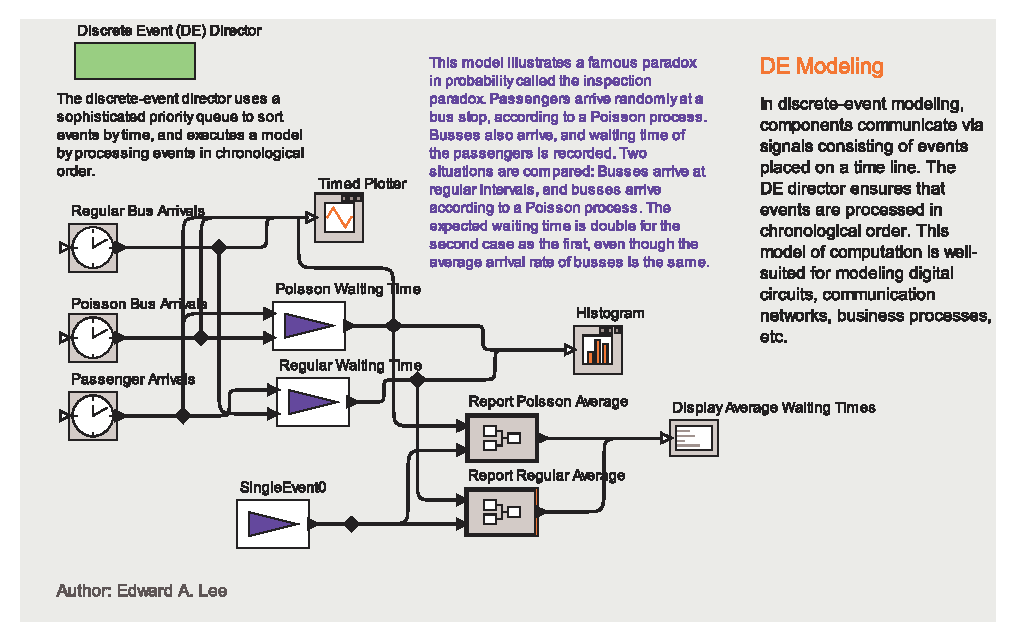
\includegraphics[width=3.5in]{figure.eps}
  \end{center}

  \caption{\small Figure caption. To get a figure to span two
      columns, use the environment figure* rather than figure.}
  \label{fig-label}
\end{figure}

\section{Using \LaTeX with EPS Figures}

This is a sample document for use with latex and dvipdfm, which is
a program that is included with the Miktex distribution
that produces PDF files from DVI files, which are produced by \LaTeX.
To run \LaTeX on this file, you need the following files:
\begin{enumerate}
\item templateEPS.tex (this file)
\item figure.eps (the figure file)
\item simpleConference.sty (style file)
\item refs.bib (bibiliography file)
\end{enumerate}
\noindent
To create a PDF file, execute the following commands:
\begin{enumerate}
\item latex templateEPS
\item bibtex templateEPS
\item latex templateEPS
\item latex templateEPS
\item divpdfm templateEPS
\end{enumerate}
\noindent
Yes (strangely) it is necessary to run latex three times.
The result will be a PDF file (plus several other files that \LaTeX
produces).  You will need a mechanism, of course, for executing
commands on the command line. If you are using Windows, I recommend
installing Cygwin and using its bash shell.

The figure \ref{fig-label} is created from Vergil, the visual
editor for Ptolemy II models \cite{PtolemyVol1:04}, by first
creating an EPS printer and printing to it, then using Ghostscript
to set the bounding box of the resulting EPS file.

\bibliographystyle{abbrv}
\bibliography{refs}
\end{document}
